\documentclass{beamer}

\mode<presentation> {
  \usetheme{Madrid}
  \setbeamercovered{transparent}
}

\usepackage[czech]{babel}
\usepackage[utf8]{inputenc}
\usepackage{graphicx}
\usepackage{hyperref}
\usepackage{multicol}
\usepackage{mathtools}


\title{Bezeztrátová komprese obrazu}
\author{Drahomír Dlabaja}
\institute[xdlaba02]{Vysoké učení technické v Brně}
\date{\today}

\begin{document}

\begin{frame}
  \titlepage
\end{frame}

\begin{frame}
  \center
  \frametitle{Kompresní řetězec}
  \begin{columns}
    \begin{column}{0.4\textwidth}
      \LARGE
  \begin{enumerate}
  \item Subtract green
  \item Paeth++
  \item MTF
  \item BWT
  \item CABAC
  \end{enumerate}
  \end{column}
  \begin{column}{0.6\textwidth}
    \begin{figure}
      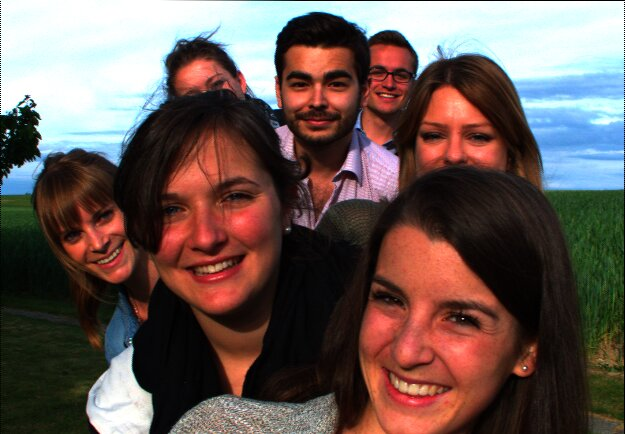
\includegraphics[width=\textwidth]{friends.jpg}
    \end{figure}
\end{column}
\end{columns}
\end{frame}

\begin{frame}
  \center
  \frametitle{Subtract green}
  \begin{figure}
    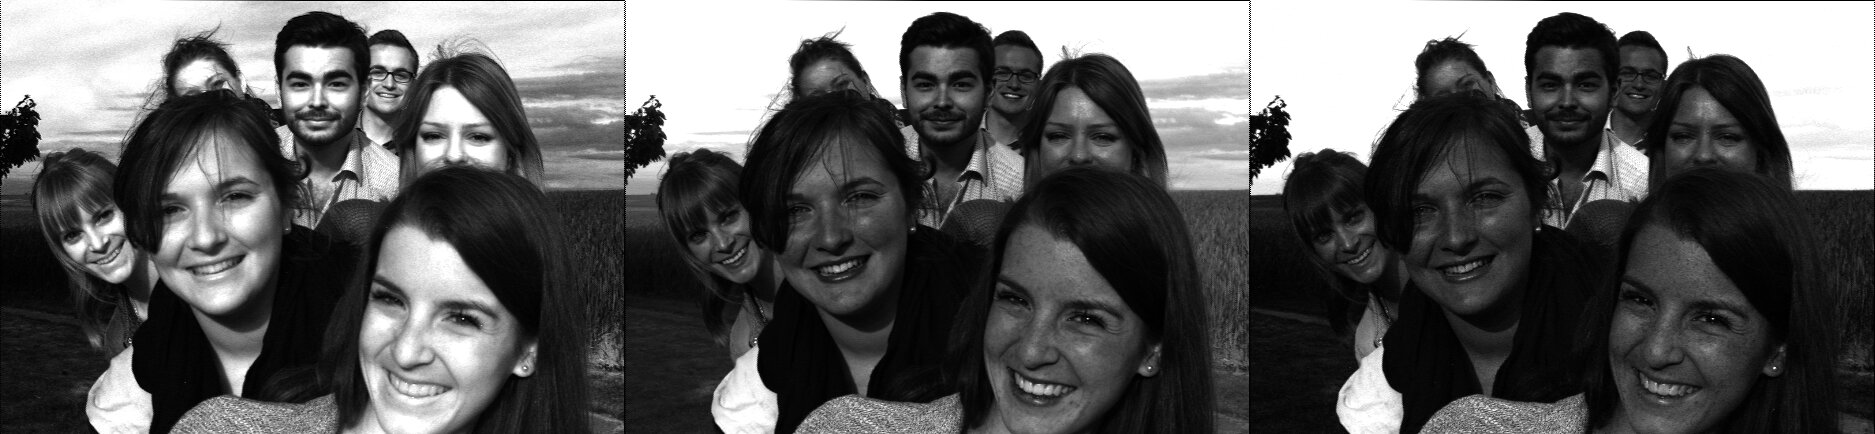
\includegraphics[width=\textwidth]{friends_orig.jpg}
  \end{figure}
  $[R, G, B] \rightarrow [R - G, G, B - G]$
  \begin{figure}
    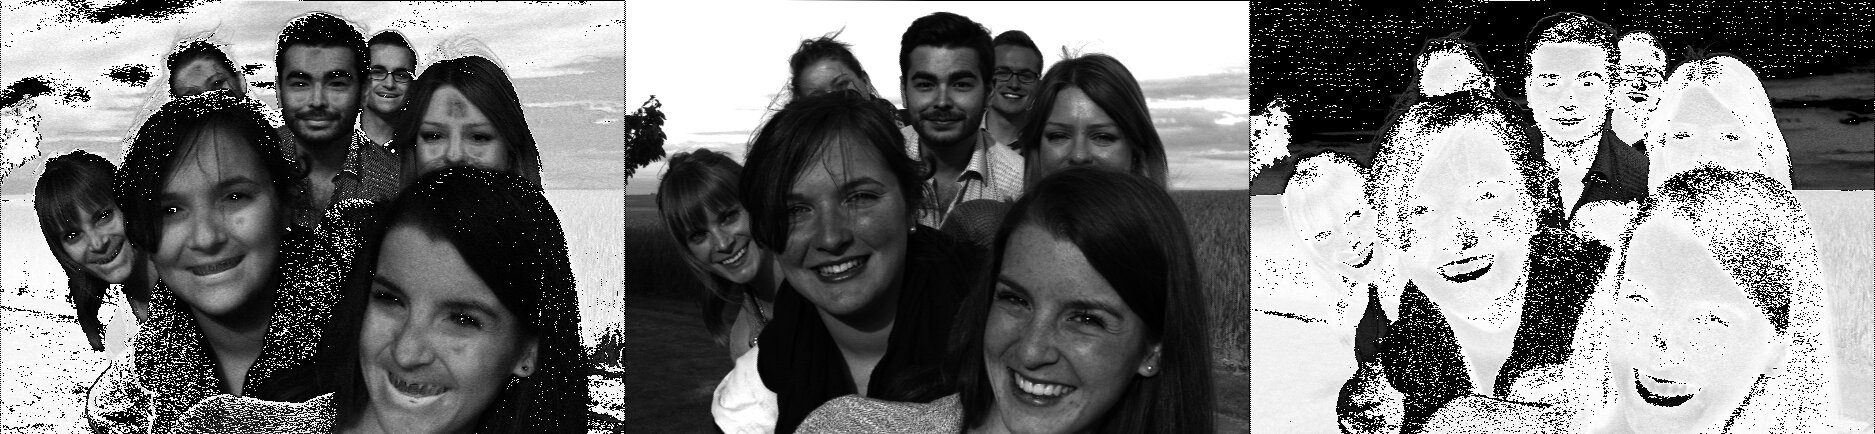
\includegraphics[width=\textwidth]{friends_transformed.jpg}
  \end{figure}
\end{frame}

\begin{frame}
  \center
  \frametitle{Modifikovaný Paethův prediktor}
  \begin{columns}
    \begin{column}{0.5\textwidth}
     \begin{figure}
       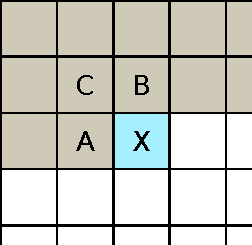
\includegraphics[height=0.4\textheight]{prediction.pdf}
     \end{figure}
    \end{column}
    \begin{column}{0.5\textwidth}
      \begin{align*}
        \begin{split}
        p &= A + B - C\\
        p_a &= |p - A|\\
        p_b &= |p - B|\\
        p_c &= |p - C|\\
        \Aboxed{p_\mathrm{avg} &= \left|p - \frac{(A + B)}{2}\right|}\\
        p_x &= \mathrm{min}\{p_a, p_b, p_c, \boxed{p_\mathrm{avg}}\}
      \end{split}
    \end{align*}

\end{column}
  \end{columns}
\end{frame}

\begin{frame}
  \center
  \frametitle{Modifikovaný Paethův prediktor}
  Funguje líp pro plynulé obrázky.\\[1em]
  \begin{figure}
  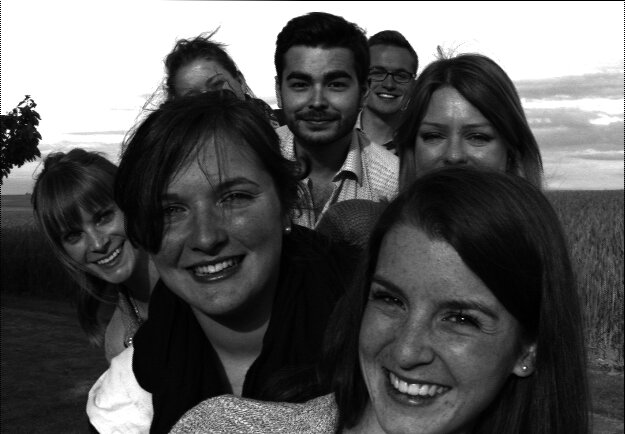
\includegraphics[width=.4\textwidth]{friends_green.jpg}
  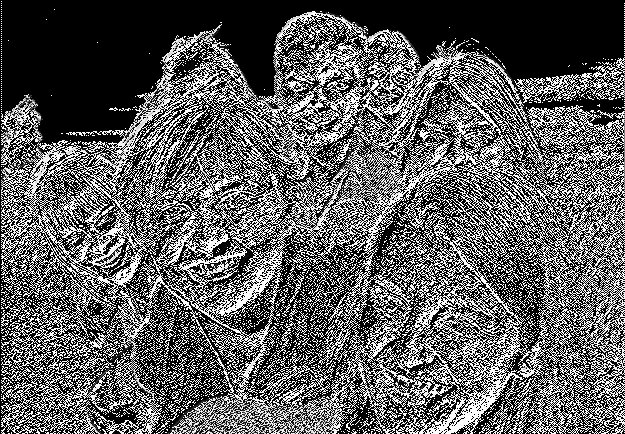
\includegraphics[width=.4\textwidth]{friends_green_pred.jpg}
  \end{figure}
  Hodně bílé a černé, málo odstínů šedé.
\end{frame}

\begin{frame}
  \center
  \frametitle{Burrows-Wheelerova transformace}
  Generuje takovou permutaci, kde se stejné symboly nachází blízko sebe.\\[1em]
  \begin{figure}
  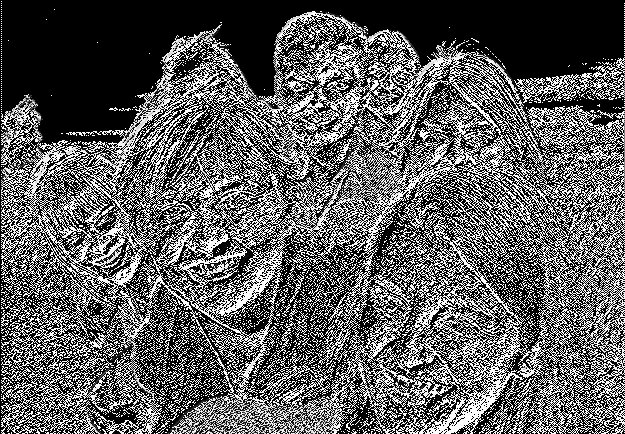
\includegraphics[width=.4\textwidth]{friends_green_pred.jpg}
  
\includegraphics[width=.4\textwidth]{friends_bwt.jpg}
  \end{figure}
  Využívá entropie vyšších řádů v datech.
\end{frame}

\begin{frame}
  \center
  \frametitle{Move-to-front transformace}
  Pokud se stejné symboly nachází blízko sebe, generuje malá čísla.\\[1em]
  \begin{figure}
  
\includegraphics[width=.4\textwidth]{friends_bwt.jpg}
  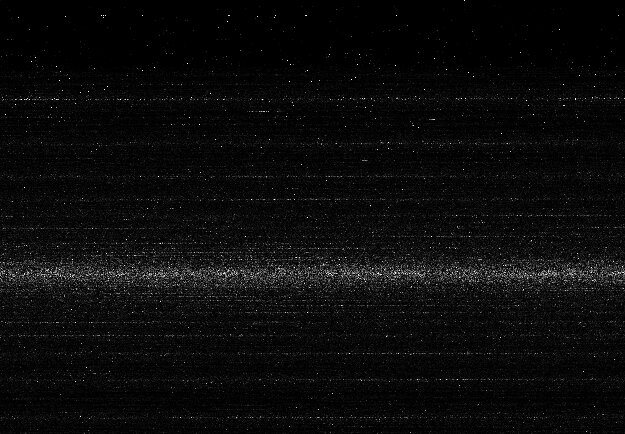
\includegraphics[width=.4\textwidth]{friends_mtf.jpg}
  \end{figure}
  V projektu byla použita \textit{sticky} varianta s koeficientem \textit{0,9}.
\end{frame}

\begin{frame}
  \center
  \frametitle{Kontextově-adaptivní binární aritmetické kódování}
  Binarizace unárním kódováním. Pro každý bit jeden kontext.\\[1em]
  \begin{figure}
  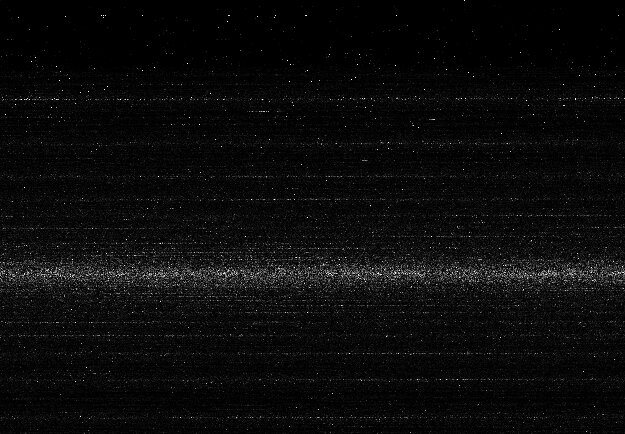
\includegraphics[width=.4\textwidth]{friends_mtf.jpg}
  
\includegraphics[width=.4\textwidth]{friends_cabac.jpg}
  \end{figure}
  Rychlé a jednoduché pro malá čísla.
\end{frame}

\begin{frame}
  \center
  \frametitle{Bitrate}
  \begin{figure}
    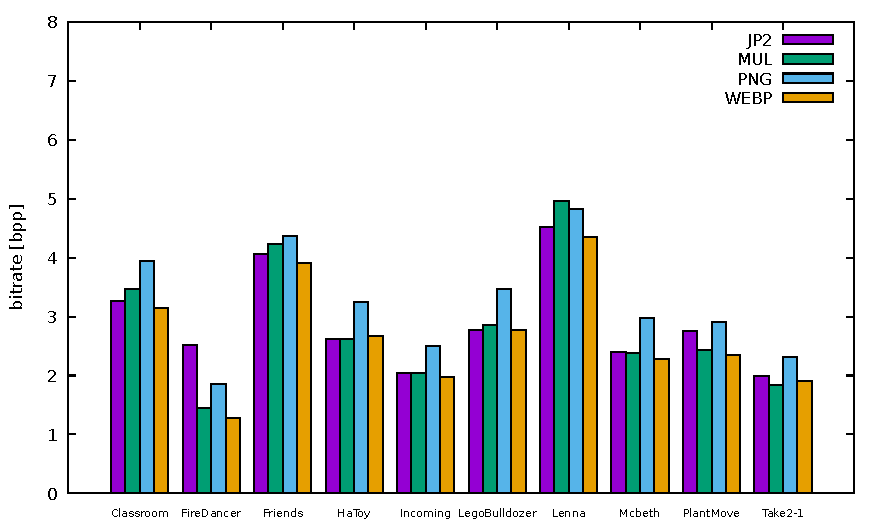
\includegraphics[width=\linewidth]{bitrate.pdf}
  \end{figure}
\end{frame}

\begin{frame}
  \center
  \frametitle{Dekomprese}
  \begin{figure}
    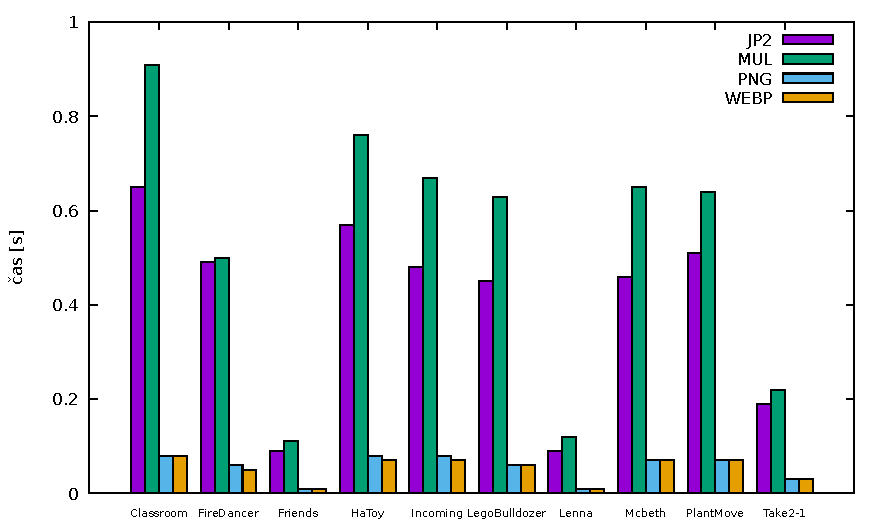
\includegraphics[width=\linewidth]{decompress_time.pdf}
  \end{figure}
\end{frame}

\begin{frame}
  \center
  \frametitle{Komprese}
  \begin{figure}
    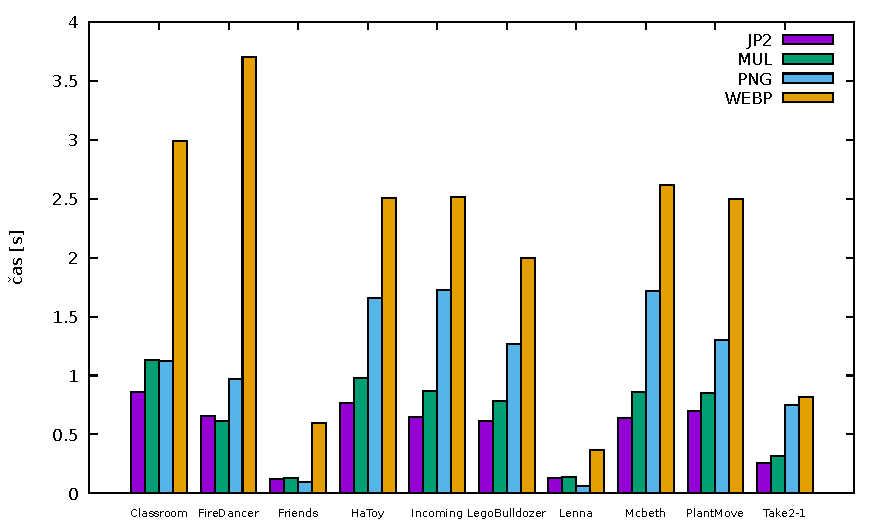
\includegraphics[width=\linewidth]{compress_time.pdf}
  \end{figure}
\end{frame}

\end{document}
